\documentclass[%
reprint,
%superscriptaddress,
%groupedaddress,
%unsortedaddress,
%runinaddress,
%frontmatterverbose,
%preprint,
%showpacs,preprintnumbers,
%nofootinbib,
%nobibnotes,
%bibnotes,
amsmath,
amssymb,
aps,
pra,
%prb,
%rmp,
%prstab,
%prstper,
%floatfix,
showkeys
]{revtex4-1}

\renewcommand{\figurename}{Figure}
\renewcommand{\tablename}{Table}

\usepackage[utf8]{inputenc}
\usepackage{colortbl}
\usepackage{graphicx}
\usepackage{hyperref}
\usepackage{ulem}

%\usepackage{epstopdf}

\usepackage{feynmp}
\DeclareGraphicsRule{*}{mps}{*}{}

\makeatletter
\def\endfmffile{%
\fmfcmd{\p@rcent\space the end.^^J%
        end.^^J%
        endinput;}%
\if@fmfio
   \immediate\closeout\@outfmf
\fi
\ifnum\pdfshellescape=\@ne
   \immediate\write18{mpost \thefmffile}%
\fi}
\makeatother

\begin{document}


% Use the \preprint command to place your local institutional report
% number in the upper righthand corner of the title page in preprint mode.
% Multiple \preprint commands are allowed.
% Use the 'preprintnumbers' class option to override journal defaults
% to display numbers if necessary
%\preprint{}

%Title of paper
\title{PhD Progress 18 Months Report}

% repeat the \author .. \affiliation  etc. as needed
% \email, \thanks, \homepage, \altaffiliation all apply to the current
% author. Explanatory text should go in the []'s, actual e-mail
% address or url should go in the {}'s for \email and \homepage.
% Please use the appropriate macro foreach each type of information

% \affiliation command applies to all authors since the last
% \affiliation command. The \affiliation command should follow the
% other information
% \affiliation can be followed by \email, \homepage, \thanks as well.
\author{João Pela}
\email[]{joao.pela@cern.ch}
%\homepage[]{Your web page}
%\thanks{}
%\altaffiliation{}
\affiliation{Imperial College London}

%Collaboration name if desired (requires use of superscriptaddress
%option in \documentclass). \noaffiliation is required (may also be
%used with the \author command).
%\collaboration can be followed by \email, \homepage, \thanks as well.
%\collaboration{}
%\noaffiliation

\date{\today}

\begin{abstract}
This is the 18 month report on my PhD progress. Theoretical and experimental motivations are presented for the analysis
in which I am involved at the Compact Muon Solenoid experiment, the standard model Higgs on the $\gamma\gamma$ decay 
channel analysis and vector boson fusion produced Higgs with invisible decay products analysis. A summary of the 
service work already performed is also made.
\end{abstract}

% insert suggested PACS numbers in braces on next line
%\pacs{}
% insert suggested keywords - APS authors don't need to do this
\keywords{Experimental high energy physics, trigger systems and data acquisition}

%\maketitle must follow title, authors, abstract, \pacs, and \keywords
\maketitle

\setlength{\unitlength}{1mm}

\section{Introduction}

The current knowledge on the field of particle physics is summarized in the standard model (SM). It is known that
this model is incomplete without the inclusion of a spontaneous symmetry breaking mechanism that would explain
the observation that the electroweak bosons (the W and Z particles) have mass. The easiest way to introduce such
a mechanism is with the Higgs mechanism, which suggests the presence of a new particle, the Higgs boson.

After 2 years of successful operation the experiments built on the Large Hadron Collider (LHC) at
European Organization for Nuclear Research (CERN) located near Geneva, Switzerland observed of
a new boson.

The Compact Muon Solenoid experiment (CMS) published results where the best-fit signal strength for a SM Higgs boson 
mass hypothesis of 125 $GeV$ is $\sigma_{SM}=0.87\pm0.23$. The excess is most significantly seen in the $\gamma\gamma$ 
and in the ZZ decay channel, which together are the channels with best mass resolution. A fit to these signals gives 
a mass of $125.3 \pm 0.4 (stat.) \pm 0.5 (syst.)$ $GeV$. The decay to two photons indicates that the new particle is 
a boson with spin different from one\cite{article:CMS-HIG-12-028}.

The ATLAS collaboration also presented simultaneously similar results and claim of a new neutral boson
with a measured mass of $126.0 \pm 0.4 (stat.) \pm 0.4 (syst.)$ $GeV$ \cite{article:CERN-PH-EP-2012-218}.

\subsection{Higgs phenomenology}

The main processes for Standard Model Higgs production are summarized in figure \ref{table_HiggsDiagrams}.

\begin{figure}[ht]
 
\begin{tabular}{cc}
\begin{fmffile}{feynmanDiagram_GFHiggs}
\fmfframe(0,5)(0,5){
\begin{fmfgraph*}(30,20)
   \fmfleft{g1,g2} \fmfright{H'}
   \fmf{gluon}{g1,t1}
   \fmf{gluon}{g2,t2}
   \fmf{fermion,tension=0,label=$t$,label.side=left}{t1,t2}
   \fmf{fermion,label=$t$,label.side=left}{t2,H}
   \fmf{fermion,label=$\bar{t}$}{H,t1}
   \fmf{boson}{H,H'}
   \fmflabel{$H^0$}{H'}
   \fmflabel{$g_1$}{g1}
   \fmflabel{$g_2$}{g2}
\end{fmfgraph*}
}
\end{fmffile}

(1) &

\begin{fmffile}{feynmanDiagram_VBFHiggs}
\fmfframe(0,5)(0,5){
\begin{fmfgraph*}(30,20)
   \fmfleft{P1,P2} \fmfright{P1',H',P2'}
   \fmf{fermion}{P1,g1}
   \fmf{fermion}{P2,g2}
   \fmf{boson,label=$W/Z^0$,label.side=left}{g1,H}
   \fmf{boson,label=$W/Z^0$,label.side=left}{H,g2}
   \fmfdot{H,g1,g1}
   \fmf{boson,tension=0.2}{H,H'}
   \fmf{fermion}{g1,P1'}
   \fmf{fermion}{g2,P2'}
   \fmflabel{$H^0$}{H'}
   \fmflabel{$q_1$}{P1}
   \fmflabel{$q_2$}{P2}
   \fmflabel{$q_1'$}{P1'}
   \fmflabel{$q_2'$}{P2'}
\end{fmfgraph*}
}
\end{fmffile}
(2) \\
\begin{fmffile}{feynmanDiagram_ttFHiggs}
\fmfframe(0,5)(0,5){
\begin{fmfgraph*}(30,20)
   \fmfleft{g2,g1}
   \fmfright{t2',H',t1'}
   \fmf{gluon}{g2,t2}
   \fmf{gluon}{g1,t1}
   \fmf{fermion}{t2',t2}
   \fmf{fermion,label.side=right,label=$t$}{t2,H}
   \fmf{fermion,label.side=right,label=$\bar{t}$}{H,t1}
   \fmf{fermion}{t1,t1'}
   \fmf{boson,tension=0.5}{H,H'}
   \fmflabel{$H^0$}{H'}
   \fmflabel{$g_1$}{g1}
   \fmflabel{$g_2$}{g2}
   \fmflabel{$t$}{t1'}
   \fmflabel{$\bar{t}$}{t2'}
\end{fmfgraph*}
}
\end{fmffile}
(3) &

\begin{fmffile}{feynmanDiagram_WZstrahlung}
\fmfframe(0,5)(0,5){
\begin{fmfgraph*}(30,20)
   \fmfleft{q2,q1} \fmfright{H',V'}
   \fmf{fermion}{v1,q2}
   \fmf{fermion}{q1,v1}
   \fmf{boson,label=$W/Z$}{v1,v2}
   \fmf{boson}{v2,V'}
   \fmf{boson}{v2,H'}
   \fmflabel{$H^0$}{H'}
   \fmflabel{$W/Z$}{V'}
   \fmflabel{$q$}{q1}
   \fmflabel{$\bar{q}$}{q2}
\end{fmfgraph*}
}
\end{fmffile}
(4)

\end{tabular}
\label{table_HiggsDiagrams}
\caption{Main processes for standard model Higgs production ordered by highest cross section at the LHC. (1) gluon 
fusion,(2) vector boson fusion, (3) $t\bar{t}$ fusion and (4) $W/Z$ associated production.}
\end{figure}

The respective cross sections for each production process can be found in figure \ref{figure_SMHiggs_XSec}
\cite{Takahashi:1019873}. It can be seen that the gluon fusion (GF) is the leading process by almost one order of
magnitude higher than vector boson fusion (VBF) which is the second most frequent process in the currently allowed 
experimental mass range for a Standard Model Higgs Boson. Both $t\bar{t}$ fusion and weak boson associated productions 
have cross sections more than one order of magnitude lower than VBF in the same mass range.

\begin{figure}[ht]
\centering
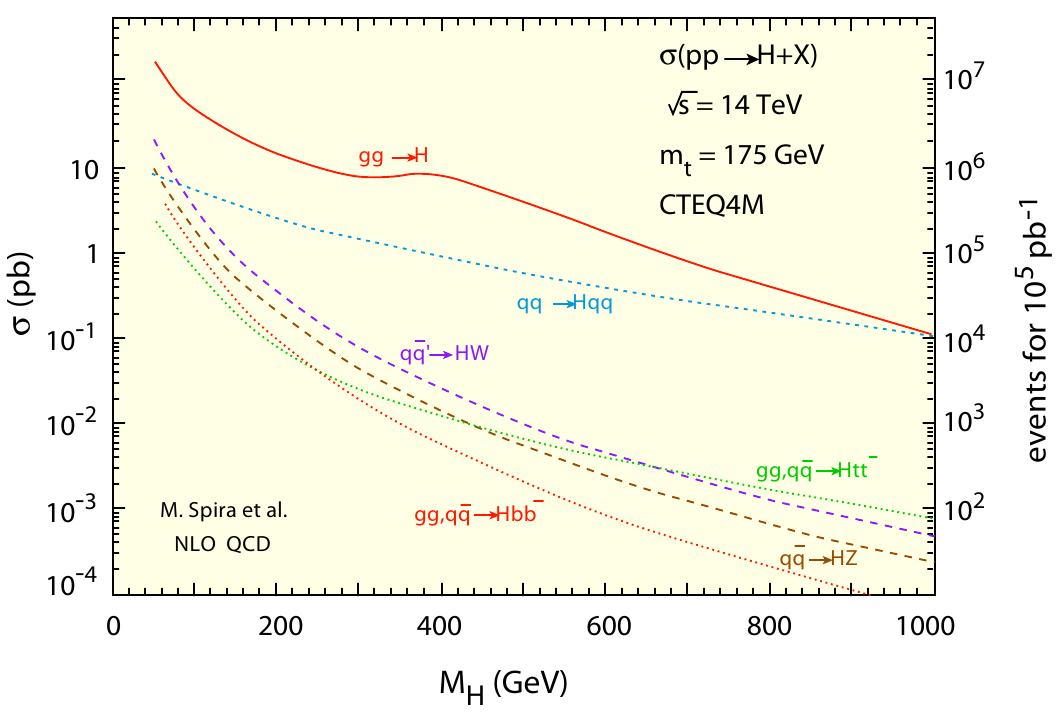
\includegraphics[width=0.45\textwidth]{img/SMHiggs_XSec.png}
\caption{Theoretical prediction of standard model Higgs productions cross sections for a $\sqrt(s)=14$ $TeV$
and assuming $m_{top}=175$ $GeV$.}
\label{figure_SMHiggs_XSec}
\end{figure}

The Higgs boson will then decay with different probabilities to different objects depending on its mass; a plot
of these probabilities can be found at figure \ref{figure_SMHiggs_BR} \cite{Takahashi:1019873}.

\begin{figure}[ht]
\centering
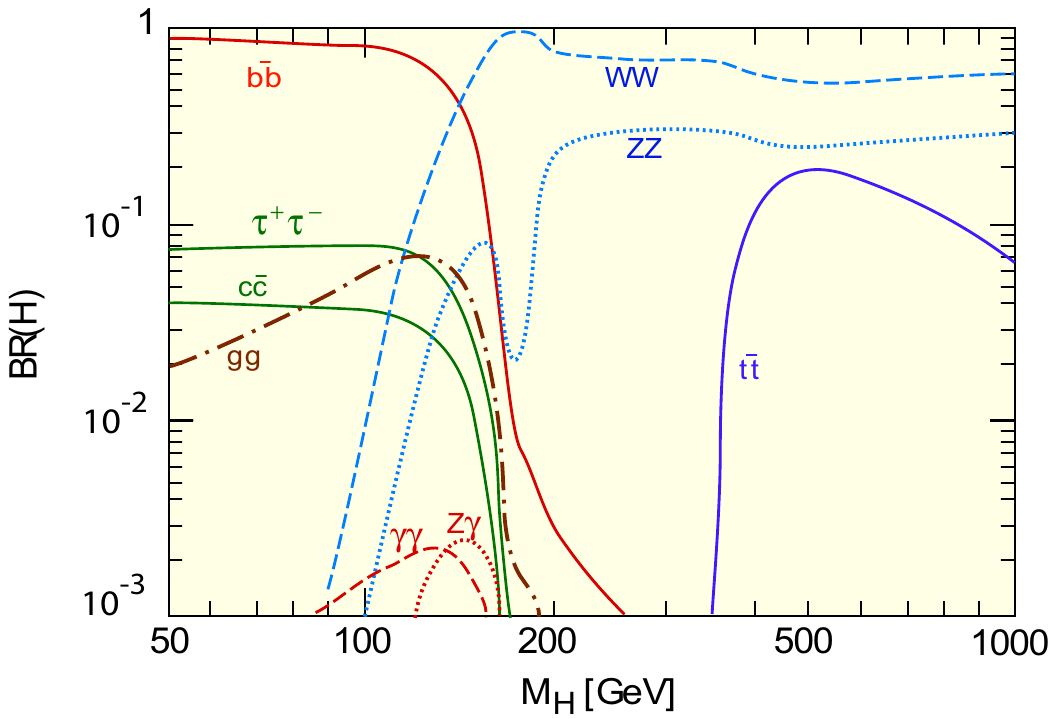
\includegraphics[width=0.45\textwidth]{img/SMHiggs_BR.png}
\caption{Theoretical prediction of standard model Higgs branching rations as a function of its mass.}
\label{figure_SMHiggs_BR}
\end{figure}

\subsection{Higgs to \texorpdfstring{$\gamma\gamma$}{gamma-gamma}}

The $H \rightarrow \gamma\gamma$ channel main production mechanism is gluon fusion. This process compared with the 
other possible production mecanisms and decays is the one that presents the biggest potential for discovery at low
masses, since its clean signature and amount of background on the signal area make this channel the most promising.

In the $H \rightarrow \gamma\gamma$ analysis a search is made for a narrow peak in the diphoton invariant mass
distribution in the range 110–150 GeV. This signal is sitting on a large irreducible background from QCD production 
of two photons and reducible background where one or more of the reconstructed photons originate from 
misidentification of jet fragments.

\subsection{Vector boson fusion Higgs to invisible}

The first theoretical motivations for looking for VBF Higgs events is obviosly to observe and measure its
cross section and each of the branching ratios for its decays. We can then calculate its coupling to the
weak bosons and to fermions (including the leptonic sector via $\tau\bar{\tau}$). From the couplings, we may be able 
to differentiate between a SM Higgs or beyond the standard model (BSM) Higgs like one of the super symmetric
incarnations of this boson\cite{article:Duhrssen:2004cv,article:Zeppenfeld:2000td}. Also for models where the Higgs 
would only decay invisibly, VBF is the primary discovery channel.

From the experimental point of view, we can see from figure \ref{figure_SMHiggs_XSec} that VBF has a cross section
one order of magnitude lower than GF, but we should notice from diagram 2 in figure \ref{table_HiggsDiagrams} that
there are two forward jets produced along with the Higgs and we can use them for tagging. 

Also, we can profit from the lack of colour exchange between the interacting quarks which will result in low hadronic activity in the
central rapidity region coming from the main interaction. Since the Higgs visible decay products (if any) are most 
likely produced in the central rapidity region, this means that they will be likely isolated from the forward jets 
thus allowing better reconstruction/identification efficiency which should allow easier study of the Higgs properties.

In the case of a invisible decay we can profit from the large Z to invisible decay branching ratio. On the other hand
we do not have the Higgs decay products to reconstruct its mass, so we have to rely only on the missing energy and 
tagged jets to identify this events.

\section{Experimental introduction}

\subsection{Large Hadron Collider}

The Large Hadron Collider (LHC) is at this moment the world's largest and highest-energy particle accelerator
in activity. It was built in a 27 kilometer circular tunnel, at an average depth of around 100 meters, under the
Franco-Swiss border near Geneva, Switzerland\cite{Bruning:2004ej}.

The LHC is a synchrotron machine designed to accelerate and collide two opposing particle beams of particles.
Particles are injected into the machine in bunches, which can be composed of protons or lead nuclei. For
protons the maximum nominal energy that can be achieved per beam is 7 $TeV$, which represents 14 $TeV$ in the
center of mass frame for a single proton-proton collision. For lead nuclei a maximum nominal energy of
574 $TeV$ per nucleus (2.76 $TeV$ per nucleon) per beam is planned. The running conditions for proton collisions
during 2012 are 8 $TeV$ center of mass energy, with an initial average number pile up collisions
of the order of 28 and a delivering instant luminosity of the order of $5 \times 10^{33}$ $cm^{-2}s^{-2}$

\subsection{Compact Muon Solenoid}

The Compact Muon Solenoid experiment (CMS) is a general purpose experiment that is an integrating part of the LHC
program. It was designed to study the collisions of two intersecting proton beams in its center \cite{article:CMSTDRv12006}.
This detector was planned with the intention of studying a broad spectrum of physics processes and is made of several
subsystems, each one designed to take advantage of some characteristics of the particles produced in order to
measure their energy, momentum and charge. The detector has classical onion structure with several layers. Starting
from the collision point outwards we have: pixel system, tracker system, electromagnetic calorimeter, 
hadronic calorimeter, magnet, muon systems and return yoke.

At nominal conditions, forty million collisions are produced in a single second and it would be impossible to
register all of them. As almost all collisions are uninteresting, the solution is to have some kind of event selection
already in the machine so we would only save the most interesting events. This is the role of the trigger system,
which over two levels, each one with more information of what happened, reduces the number of events to a
manageable rate.

The overall dimensions of CMS detector are a length of 21.6 $m$, a diameter of 14,6 $m$, and total weight of
12500 $tons$.

\subsection{Trigger}

During 2012 LHC is being run with $50$ $ns$ bunch separations leading to a maximum bunch crossing rate of 20 $MHz$. 
Data from only about $10^3$ $events/sec$ can be written to archival media; hence, the trigger system has to achieve a
rejection factor of $\sim 2 \times 10^5$ by selecting what may be the most interesting events. The CMS trigger and data 
acquisition system consists of: the detector electronics, the Level-1 trigger processors (calorimeter, muon, and global), 
the readout network, and an online event filter system (processor farm) that executes the software for the High-Level 
Trigger (HLT).

\subsection{Level 1 trigger}

The size of the LHC detectors and the underground caverns imposes a minimum transit time for signals from
the front-end electronics to reach the services cavern housing the Level-1 trigger logic and return back to the
detector front-end electronics. The total time allocated for the transit and for reaching a decision to keep or
discard data from a particular beam crossing is 3.2 $\mu s$. During this time, the detector data must be held in
buffers while trigger data is collected from the front-end electronics and decisions are reached. This decision
allows to discard a large fraction of events while retaining the small fraction of interactions of interest (nearly
1 crossing in 1000) at hardware level. Of the total latency, the time allocated to Level-1 trigger calculations
is less than 1 $\mu s$.

\subsubsection{Level 1 Trigger Data Quality Monitoring}

The CMS Experiment developed a central data quality monitoring (DQM) System. This system provides online monitoring 
for the experiment, offline data validation/certification as well as other monitoring capabilities.

The online DQM system runs in real time in parallel with the data taking and produces plots based on the analysis of a
fraction (typically 5\%) of the events recorded in stream A (data for prompt reconstruction). The results are shown in 
an online interface accessible with a normal internet browser.

The offline DQM system runs over the full data in the next few days after it has been recorded and produces plots with 
the full statistics available, thus providing a good handle to determine data quality and provide certification.

Like other systems on CMS the level 1 trigger also has online and offline DQM areas which are crucial to monitor its 
proper functioning and provide information for data certification specific for the level 1 trigger.

\section{Data Analysis}

\subsection{Vector Boson Higgs to Invisible}

\subsubsection{VBF Signature at CMS}

The VBF SM Higgs signature main characteristic is the presence of two forward jets associated with the Higgs 
(see diagram 2 in figure \ref{table_HiggsDiagrams}). These two forward jets have a reasonably $p_T$ ($\gtrsim30$ $GeV$), 
high $\Delta\eta$ separation between them ($\gtrsim 3)$ and low $\Delta\phi$ ($\lesssim 2.5$).
The dijet pair also has a high invariant mass since it will be produced back-to-back to the Higgs boson. Because there
is no color exchange between the incoming quarks, the hadronic activity between the jets is suppressed. On the other
hand, the Higgs decay products, if any, will be located at the central rapidity area which will could be easier to 
study because of the lower hadronic activity coming from the main interaction already 
described\cite{article:Dokshitzer:1991he}. 

To illustrate this separation of the SM Higgs decay products lets look at VBF Higgs decay to a pair of $\tau$.
The distribution of the pseudo-rapidity for both forward jets and two $\tau$ coming from SM Higgs decay of simulated 
events at the CMS detector can be found in figure \ref{figure_VBF_HToTauTau_ObjectsRapidityGap}.

\begin{figure}[ht]
\centering
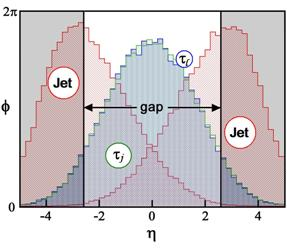
\includegraphics[width=0.45\textwidth]{img/ObjectsRapidityGap.jpeg}
\caption{Simultaneous plot of the $\eta$ coordinate of both forward jets and the $\tau\bar{\tau}$
produced from simulated VBF Higgs decay. Super-imposed with 4 circles showing the possible positions of these 4
objects in a hypothetical event.}
\label{figure_VBF_HToTauTau_ObjectsRapidityGap}
\end{figure}

The CMS detector is ideal for these type of searches since it is an $4\pi$ hermetic detector with calorimeter coverage
from -5 to 5 in pseudo-rapidity. It also has very good capabilities of particle measurement and identification which 
can be used to identify the forward jets and Higgs decay products or in case of an invisible decay, compute the 
resulting missing transverse energy. An event display of a simulated Standard Model Higgs (which then decays to 
$\tau\bar{\tau}$) produced via VBF can be found at figure \ref{figure_EventDisplay_VBF_HToTauTau_El-Had}.

\begin{figure}[ht]
\centering
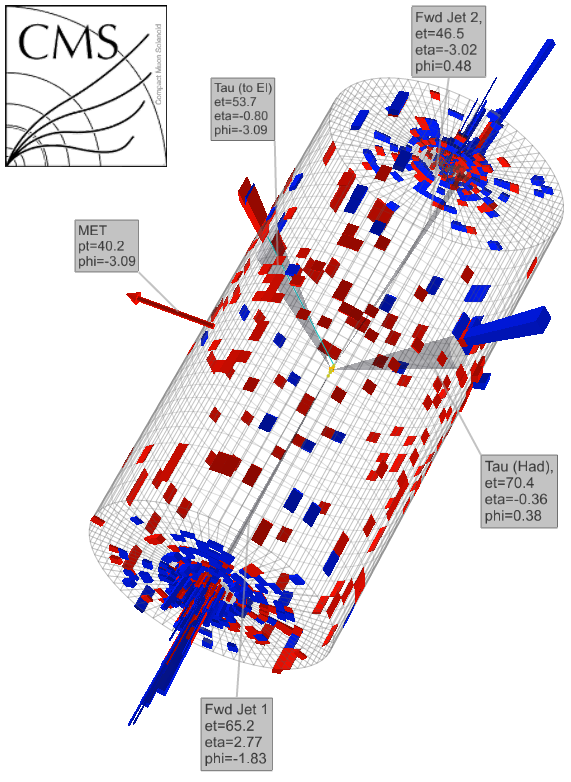
\includegraphics[width=0.45\textwidth]{img/EventDisplay_VBF_HToTauTau_El-Had.png}
\caption{Event display of a simulated event where a standard model Higgs is produced via vector boson fusion
which then decays to $\tau\bar{\tau}$, which in turn decay leptonically to electron (left) and hadronically (right).}
\label{figure_EventDisplay_VBF_HToTauTau_El-Had}
\end{figure}

\subsubsection{L1 Trigger Studies}

The first step of any analysis is defining or selecting a trigger to collect data. This trigger should have a high
signal efficiency while recording an acceptable background.

At the beginning of 2012 the possibility of recording data without promptly reconstruct it was introduced, thus 
allowing to record up to 1500 $Hz$ of data where only 300 $Hz$ are promptly reconstructed. This is now know as
\textit{parked data}, and it will only be reconstructed after the beginning of \textit{Long Shutdown 1} in 2013.

A study was initiated on the possibility to use this extra bandwidth to make a set of triggers that would cover 
record VBF events regardless of final state. 

\subsubsection{Invisible Higgs trigger}

I have been involved in a study of a CMS level 1 trigger algorithm with the objective of efficiently selecting
VBF higgs to invisible decays. This study was based on real data from the high pileup special run taken late 2011
and was aimed at making a proposal for a viable trigger algorithm to be used in the 2012 proton run.
The algorithm was based on selecting missing transverse energy (MET) and two jets that would pass the test
$\eta_{jet1}\times\eta_{jet2}<0$ and would have a separation of $\Delta\eta_{jj}>3$. A possible additional cut
was also studied: a restriction on $\Delta\phi_{jj}$, and tested points were not cut, $<2.5$, $<2.1$ and $<1.8$. 
For the conditions expected at this point for early 2012 (i.e. instant luminosity of $5e33$ and $<PU>=28$) two tables 
were produced reporting the cuts necessary to achieve a given rate threshold, one assuming fixed dijet $E_\bot$ cut 
and varying MET (table \ref{table_5E33_PU28_fixedDijet}) and another assuming fixed MET cut and varying $E_\bot$ 
(table \ref{table_5E33_PU28_fixedMET}).

\begin{table}
\begin{tabular}{|c||c|c|c|c|}
\hline
\multicolumn{5}{|c|}{MET [GeV] ($E_\bot(jj)>20$ [GeV])} \\
\hline
$\Delta\phi$ & no cut & 2.5 & 2.1 & 1.8 \\
\hline
10kHz        &     32 &  32 &  32 &  32 \\
5kHz         &     35 &  35 &  35 &  35 \\
\cellcolor{green}2kHz &\cellcolor{green}      41 &  41 &  41 &  41 \\
1kHz         &     47 &  47 &  47 &  46 \\
500Hz        &     54 &  54 &  54 &  53 \\
\hline
\end{tabular}
\caption{Cut thresholds to apply to MET assuming fixed dijet $E_\bot>20$ [GeV] to obtain specific L1 rates forced
instant luminosity of $5e33$ and $<PU>=28$. Highlighted in green is the working point suggested to the Tigger
Studies Group for the L1 trigger.}
\label{table_5E33_PU28_fixedDijet}
\end{table}

\begin{table}
\begin{tabular}{|c||c|c|c|c|}
\hline
\multicolumn{5}{|c|}{$E_\bot(jj)$ [GeV] ($MET>30$ [GeV])} \\
\hline
$\Delta\phi$ & no cut & 2.5 & 2.1 & 1.8 \\
\hline
10kHz        &     28 &  28 &  24 &  24 \\
5kHz         &     32 &  32 &  32 &  32 \\
\cellcolor{green} 2kHz         &\cellcolor{green}      52 &  48 &  44 &  44 \\
1kHz         &     68 &  68 &  64 &  64 \\
500Hz        &     92 &  92 &  88 &  88 \\
\hline
\end{tabular}
\caption{Cut thresholds to apply to dijet $E_\bot$ assuming fixed dijet $MET>30$ [GeV] to obtain specific L1 rates 
forced instant luminosity of $5e33$ and $<PU>=28$. Highlighted in green is the working point suggested to the Tigger
Studies Group for the L1 trigger.}
\label{table_5E33_PU28_fixedMET}
\end{table}

Results were used to define working points for this trigger, which were already proposed to the Trigger Studies Group
to be included on future L1 Trigger Menus. Proposed trigger options were:
\begin{itemize}
\item Dijet $E_\bot>20$ $GeV$ + fwd/bkwd + $\Delta\eta_{jj}>3$ + $MET>40$ $GeV$
\item Dijet $E_\bot>50$ $GeV$ + fwd/bkwd + $\Delta\eta_{jj}>3$ + $MET>30$ $GeV$
\end{itemize}

Further studies were made for conditions predicted for late 2012 (i.e. instant luminosity of $7e33$ and $<PU>=32$)
and can be found in tables \ref{table_7E33_PU32_fixedDijet} and \ref{table_7E33_PU32_fixedMET}.

\begin{table}
\begin{tabular}{|c||c|c|c|c|}
\hline
\multicolumn{5}{|c|}{MET [GeV] ($p_\bot(jj)>20$ [GeV])} \\
\hline
$\Delta\phi$ & no cut & 2.5 & 2.1 & 1.8 \\
\hline
10kHz        &     36 &  36 &  36 &  36 \\
5kHz         &     40 &  40 &  40 &  40 \\
2kHz         &     47 &  47 &  47 &  46 \\
1kHz         &     54 &  54 &  54 &  54 \\
500Hz        &     67 &  66 &  66 &  64 \\
\hline
\end{tabular}
\caption{Cut thresholds to apply to MET assuming fixed dijet $E_\bot>20$ [GeV] to obtain specific L1 rates forced
instant luminosity of $7e33$ and $<PU>=32$}
\label{table_7E33_PU32_fixedDijet}
\end{table}

\begin{table}
\begin{tabular}{|c||c|c|c|c|}
\hline
\multicolumn{5}{|c|}{$p_\bot(jj)$ [GeV] ($MET>30$ [GeV])} \\
\hline
$\Delta\phi$ & no cut & 2.5 & 2.1 & 1.8 \\
\hline
10kHz        &     32 &  32 &  32 &  32 \\
5kHz         &     40 &  40 &  40 &  40 \\
2kHz         &     64 &  60 &  60 &  56 \\
1kHz         &     76 &  76 &  76 &  76 \\
500Hz        &    100 & 100 &  96 &  92 \\
\hline
\end{tabular}
\caption{Cut thresholds to apply to dijet $E_\bot$ assuming fixed dijet $MET>30$ [GeV] to obtain specific L1 rates 
forced instant luminosity of $7e33$ and $<PU>=32$}
\label{table_7E33_PU32_fixedMET}
\end{table}

\subsubsection{Inclusive Higgs trigger}

It would be desirable to have a dedicated inclusive L1 trigger (i.e. Higgs decay independent). Such a trigger
would allow us to have a single trigger for all VBF signature analysis, which implies less systematics
while comparing them. Also, usually the more people using a trigger means it will become better understood by all.

By triggering only on the dijet that is tagged as the a VBF signature we therefore have no dependence on the Higgs 
decay, which means we can get all possible Higgs decays with a single trigger, even those that are predicted by 
yet to be defined models. Thus, it would be a model-independent trigger.

This trigger can also be used for a WW scattering analysis, aimed at standard model without a new symmetry 
breaking mechanism exclusion, since the signature is similar.

For such a trigger to work it would have to be based only on the forward dijet which is the defining caracteristic
of the VBF signature.
It was decided to study two variables of the dijet system: invariant mass and transverse invariant mass (MT); and an event 
variable, scalar sum of the hadronic energy (HT). For this study we always require a dijet with $\Delta\eta>3$ and we 
look at the effects of an additional cut on $\Delta\phi$, the points tested were no cut, $<2.5$, $<2.1$ and $<1.8$.

\subsubsection{Dijet invariant mass}

This variable takes advantage from the very high invariant mass of the dijet system but it is not yet implemented
on the L1 hardware but according to trigger experts it is in principle possible to implement with the current hardware.

Unfortunately, using this variable alone to is not enough. To get acceptable rates we would need to cut too high on
jet $p_\bot$ or $M_{Inv}$ losing almost all signal efficiency.

\subsubsection{Dijet transverse invariant mass}

This variable is better at suppressing QCD events, it is less pileup-dependent and has lower error associated with it
(only x-y dependence). It is also not yet implemented on the L1 Hardware but according to trigger experts it is in principle 
possible to implement with the current hardware.

This variable showed to be promising. A possible working point for a Level 1 rate
of 5kHz could be $MT>50$ $GeV$ no $\Delta\phi$ cut and dijet $p_\bot \sim 45$ $GeV$ which should give a signal
efficiency of $\lesssim70\%$ (see R. Lane 3 Months PhD Report).

\subsubsection{Event scaler sum of the transverse energy}

Theoretically, this is the best variable to separate signal from background and has the advantage of being already
implemented on L1 hardware.

This was shown to be the most promising variable. A possible working point for a Level 1 rate of 5kHz could be $HT>100$ 
$GeV$ no $\Delta\phi$ cut and dijet $p_\bot \sim 40$ $GeV$ which should give a signal efficiency of $\lesssim98\%$
(see Figures \ref{figure_PU28_5e33_RateFBDijetDEtaDPhi00HT100} and \ref{figure_sig_eff_l1_ht}).

\begin{figure}[ht]
\centering
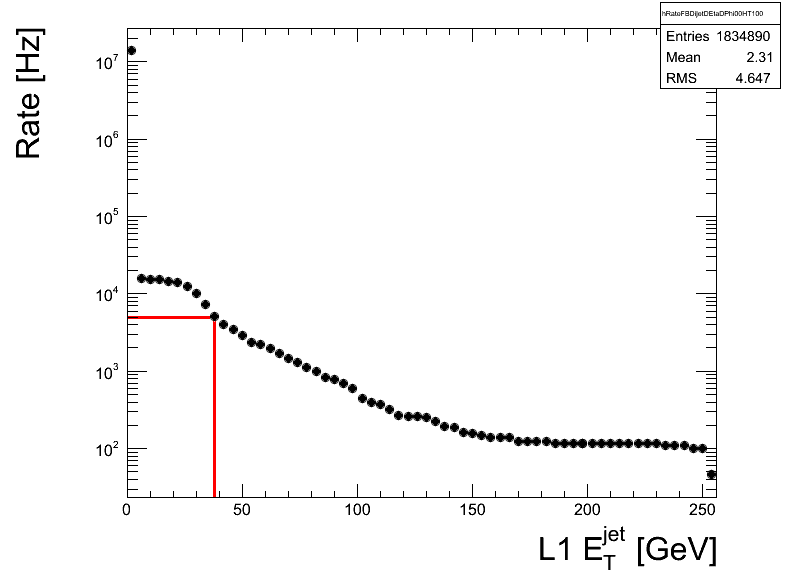
\includegraphics[width=0.45\textwidth]{img/PU28_5e33_RateFBDijetDEtaDPhi00HT100.png}
\caption{Level 1 rate as a function of dijet $p_\bot$ while selecting events with $HT>100$ $GeV$. Results based on
data from the high pileup special run taken late 2011.}
\label{figure_PU28_5e33_RateFBDijetDEtaDPhi00HT100}
\end{figure}

\begin{figure}[ht]
\centering
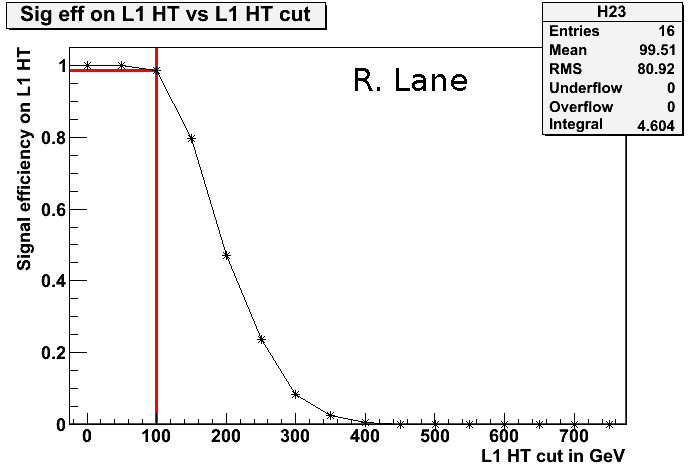
\includegraphics[width=0.45\textwidth]{img/sig_eff_l1_ht.png}
\caption{Higgs to $\tau\bar{\tau}$ signal efficiency as a function of HT cut extracted from monte carlo simulation.
Result from R. Lane.}
\label{figure_sig_eff_l1_ht}
\end{figure}

\subsection{Higgs to \texorpdfstring{$\gamma\gamma$}{gamma-gamma}}

The Higgs to $\gamma-\gamma$ analysis searches for a peak on the diphoton mass spectrum. Candidate diphoton events are 
separated into mutually exclusive categories of different expected signal-to-background ratios, based on the properties 
of the reconstructed photons and on the presence of two jets satisfying criteria aimed at selecting events in which 
a Higgs boson is produced through the VBF process. The analysis uses multivariate techniques for the selection and 
classification of the events.

\subsubsection{Background fit function choice systematics study}

In order to extract the signal yield we must perform mass fit to the background in order to estimate its contribution 
to the signal region. In the side band analysis this fit is done excluding the signal region in order to perform a 
fit unbiased by the presence of signal.

This choice of function introduces a systematic since we do not know the underlying function in the processes produce 
and smear our data. Thus, implying the need to study how much this choice changes our background estimation.
To perform this study we need to choose which candidate functions or function classes are adequate to fit our 
background. For applicability and simplicity and function classes of polynomials, exponentials and power laws were 
selected.

If we assume the we are fitting our data with function A and want to study function classes 1,2 and 3, the step of 
the study are:
\begin{enumerate}
 \item Fit A to the data excluding the signal region and obtain a signal estimation.
 \item Generate toys based on the fit made from A with the same number of events seen in data (all window).
 \item Fit each toy with every selected function from class 1, 2 and 3. Calculate the number of events in the signal 
 region. Compare the obtained value with the initial prediction of A over the data and plot them for each selected. 
 These plots should have a Gaussian distribution where the mean is the difference between A and the selected function, 
 which will contribute to the global systematic of the signal choice, and the sigma is the statistical error associated 
 from the initial dataset. An example of such plot can be seen at figure \ref{figure_SystematicAnalysis_Plot}.
 \item We can combine the plots produced in the previous step by weighting them by the $p-$value of that fit to the 
 initial data (implying that the functions that fit the data worse will have less weight).
 \item We can now extract the global mean, which is an approximation of the systematic associated with the choice of 
 function and global RMS which is an approximation of the statistical error associated with the initial data.
\end{enumerate}

\begin{figure}[ht]
\centering
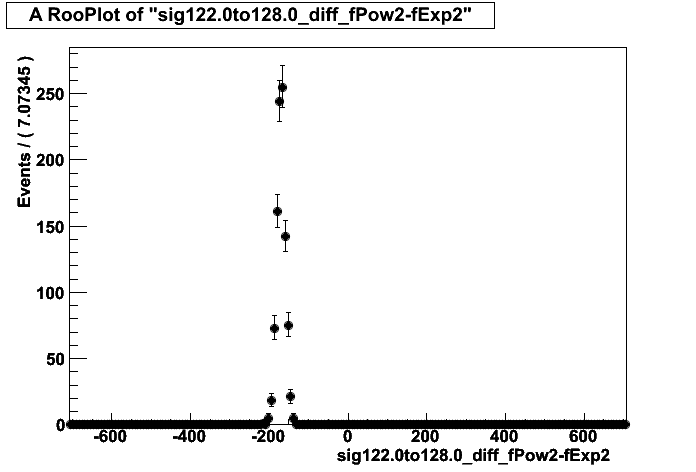
\includegraphics[width=0.45\textwidth]{img/sig122to128_Truth-fPow2_vs_fExp2.png}
\caption{Plot of the diference of extimation of background contribution on the signal area, made by fitting toys from a generating
power law of the second degree function and fitting with a exponential of the second degree. The mean for the gaussian fit to that
distribution is $-169.95\pm0.55$ (systematic error of choosing power law over exponential) and the RMS is $10.89\pm0.39$ (statistical 
error associated with the data initial statistics).}
\label{figure_SystematicAnalysis_Plot}
\end{figure}

\subsubsection{Spin analysis}

With the observation of a new boson, now the focus turns to properties measurement. One of the important properties
to measure is the spin of the new particle. We know from the decay channel where it was observed, $\gamma\gamma$ 
and $Z^0Z^0$ that it must have even value.

The SM Higgs is spin 0 but there are other models that predict particles with Spin 2 like the RS Graviton model.

To measure the spin we need to look into a variable that is sensitive to it. It was chosen to use $cos(\theta^{*})$ 
which is the angle between the diphoton on the SM Higgs rest frame and a specific z-direction.

For this feasibility study we started from the events selected by the benchmark analysis that was used for claiming 
discovery of the new boson. Specifically, events that pass the diphoton BDT cut with a score of -0.05 or more.

To determine which is the best frame to measure $cos(\theta^{*})$ we compared MC samples of SM Higgs and RS graviton. 
The following reference frames where analyzed: Collins-Soper, Helicity, Perpendicular Helicity, Gottfried-Jackson and 
Vector Addition. It was determined that the best frame to use would be the Collins-Soper, as it shows better the 
difference between the two models \ref{figure_SpinAnalysis_CosThetaStar}.

\begin{figure}[ht]
\centering
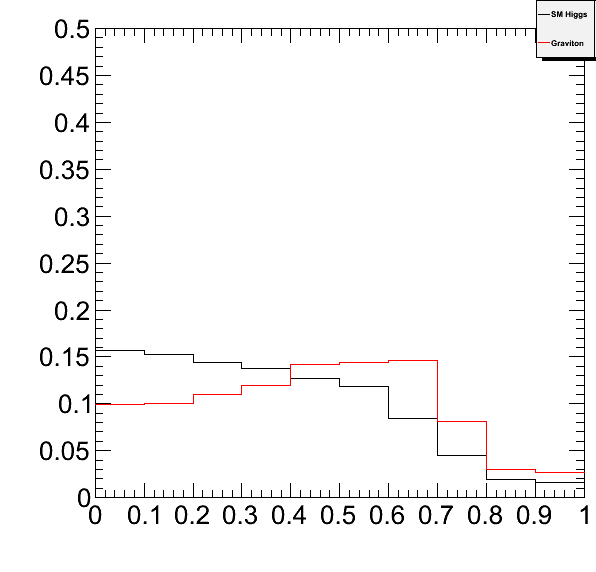
\includegraphics[width=0.45\textwidth]{img/cosThetaStar_cs_all_Norm1_SignalCompare.png}
\caption{Plot for the absolute value of $cos(\theta^{*})$ for both Monte-Carlo samples of standard model Higgs and RS graviton. 
Both distributions are normalized to 1.}
\label{figure_SpinAnalysis_CosThetaStar}
\end{figure}

It was decided to use the categories already present at the reference analysis and further split them in two by 
defining a threshold in $cos(\theta^{*})$. The split point was chosen in the crossing point of each sample 
$cos(\theta^{*})$ distribution when normalized to one, which make the sum of absolute differences between sample 
yields maximal.

Now we can create a signal model from Monte-Carlo by fitting each category, and extract signal yields from data, 
by combining the signal models with an adequate background model.

Several methods for calculating signal significance/exclusion are now being investigated, which attempt to make use 
of not only the yield but also the relative amount of signal in each bin.

\section{Service work}

At the CMS collaboration one of the requirements of authorship is to provide a given amount of \textit{service work}
for the experiment.
It is possible possible to do service work in several ways, from providing direct contribution to the operation of
the experiment to developing hardware upgrades to future implementation on the experiment itself.

My service work for 2012 is being done in two ways: by doing central shifts and development of monitoring for the
L1 trigger system.

\subsection{Central shifts}

The shifts taken were week long in the role of level 1 trigger detector on call (L1T DoC). This is the on call contact
person for the L1 trigger, which is responsible for supporting the online operation of this subsystem. In case of
any problem arising in the trigger systems, the L1T DoC provides expertise to solve the issue or passes the information
to the relevant experts.

\subsection{L1 trigger data quality monitoring}

Before I started my PhD at Imperial College, I worked as a developer for the level 1 trigger data quality monitoring
(L1T DQM). Building upon this previous experience I took over the coordination of the central L1T DQM software starting
June 2012. This role involves coordinating the L1T DQM developers in all the stages of the software cycle of the L1TDQM
cycle, from planning to deprecation.

New developers joined the L1T DQM group, for which I created a dedicated e-group where coordination and technical
information is shared. Furthermore I chair weekly meetings for the planning and discussion of the software developments.

\subsubsection{Rates monitoring}

This tool was initially developed by me during last year and now has been improved. It monitors the rate of the
lowest unprescaled single object trigger of all available L1 trigger object categories by calculating its
average cross section for each luminosity section as a function of instant luminosity and comparing this value to
fits preformed in previous runs. New developments currently include using different fits considering specific pairs of
LHC bunch filling schemes and trigger configuration key in order to ensure reference fits are done in similar conditions.

\begin{figure}[ht]
\centering
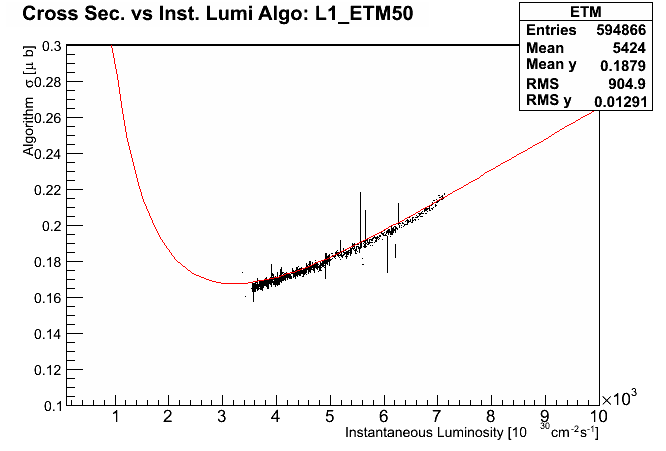
\includegraphics[width=0.45\textwidth]{img/L1TRate_L1_ETM50.png}
\caption{Monitoring plot produced by the L1TRate tool for L1 $E_T^{miss}$ object category, which is automatically
monitoring algorithm L1\_ETM50 for the run 207099. In the plots data points are the calculated trigger cross
section as a function of instant luminosity and the line is the reference fit done from previous runs.}
\label{figure_ServiceWork_L1TRate}
\end{figure}

\subsubsection{Synchronization monitoring}

This tool was initially developed by me during last year and now has been improved and debugged. It monitors
the synchronization of the lowest unprescaled single object trigger of all available L1 trigger object categories
by looking at HLT pass-through paths events (no selection at LHC to avoid bias) and looking at the 5 bunch crossing
L1 trigger information provided by the GT. The trigger records can then be compared with the published LHC bunch
structure and a fraction of in time events can be calculated. New developments include alteration in the way
information is retrieved from the database and avoiding the use of HLT pass-throughs and therefore improving statistics
by looking at events from an object category seeded by an independent object category. As an example: single muon
trigger can seed calorimeter triggers synchronization tests.

\begin{figure}[ht]
\centering
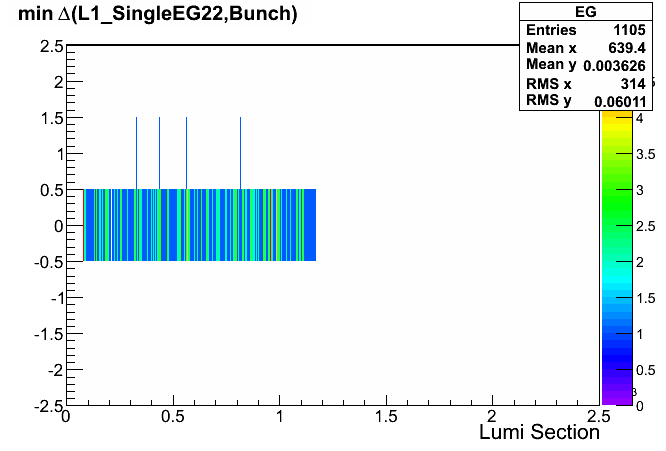
\includegraphics[width=0.45\textwidth]{img/L1TSync_L1_SingleEG22.png}
\caption{Monitoring plot produced by the L1TSync tool for L1 single electron/gamma object category, which is
automatically monitoring algorithm L1\_SingleEG50 for the run 207099. In the plots data points are the calculated
trigger cross section as a function of instant luminosity and the line is the reference fit done from previous runs.}
\label{figure_ServiceWork_L1TSync}
\end{figure}

\subsubsection{Beam Pickup for Timing for the eXperiments monitoring (BPTX)}

This tool was created during August 2012 to meet a concern of the L1 trigger management. It monitors the Beam
Pickup for Timing for the eXperiments (BPTX) system by looking at the information present at each event that 
is analyzed by the DQM system, including the 2 bunch crossings before and after the actual event that fired. Then it 
compares where the BPTX fired on those 5 bunch crossings with the LHC published bunch structure. The BPTX efficiency 
and misfire rate are calculated and the rate stability is also monitored.

\begin{figure}[ht]
\centering
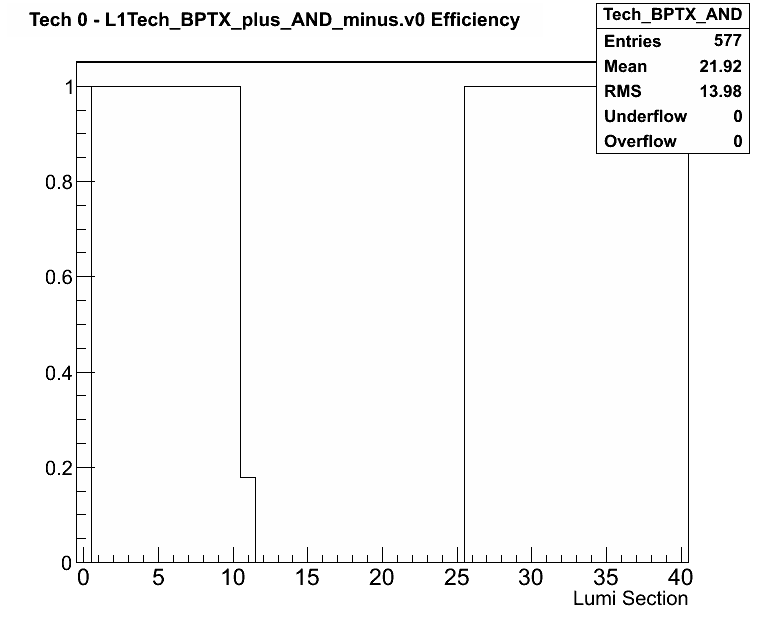
\includegraphics[width=0.45\textwidth]{img/L1TBPTX_Tech_BPTX_AND.png}
\caption{Monitoring plot produced by the L1TBPTX tool for the run 207269 where a test was executed to demonstrate that 
this tools works. In the plot the BPTX AND (technical algorithm 0) efficiency is calculated per luminosity section 
when compared with the LHC published bunch structure. The dip in efficiency corresponds to the disabling of the BPTX 
related triggers.} 
\label{figure_ServiceWork_L1TBPTX}
\end{figure}

\subsubsection{Occupancy monitoring}

This tool was developed initially by me in collaboration with a CERN summer student during last year and has been
also improved and debugged. It monitors several key occupancy plots from L1 subsystems, by making use of the natural
$\eta-\phi$ symmetry normally present. It compares each cell to the median of a strip in $\phi$ in the opposite $\eta$
side of the detector, by applying a $\chi^{2}$ like test tuned to fire when the cell is less than 10\% or more than
twice the value of the reference median. New developments include the inclusion of new plots which comply with the
tools specifications (provided by the sub-systems) and include the possibility of masking strips from the test, which 
will make the tool compare the cell with the median of the $\phi$ strip where it is included.

\begin{figure}[ht]
\centering
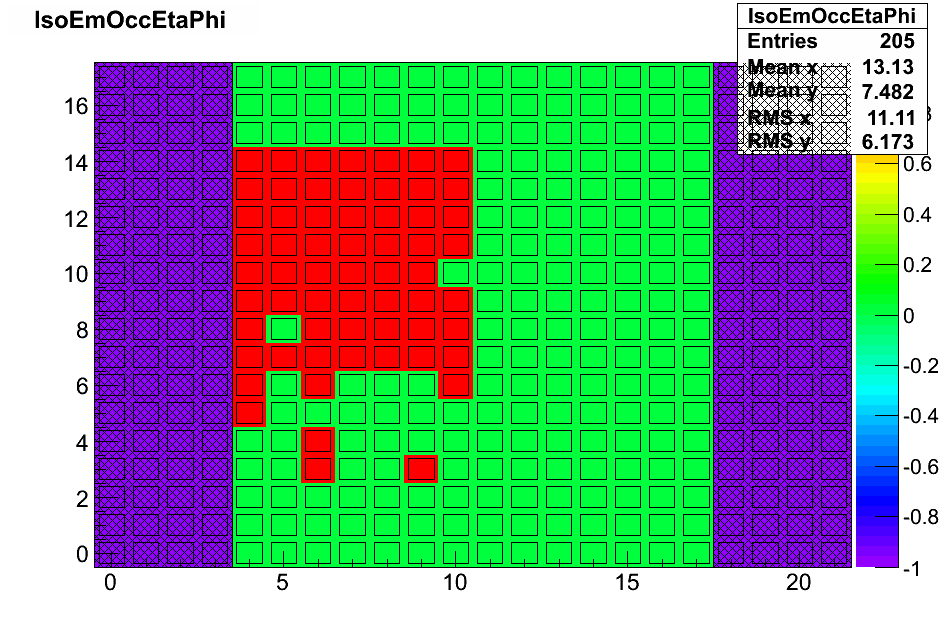
\includegraphics[width=0.45\textwidth]{img/L1TOccupancy_IsoEmOccEtaPhi.png}
\caption{Monitoring plot produced by the L1TOccupancy tool for the run 207099 while testing GCT plot for isolated
EM occupancy $\eta-\phi$. In blue are the masked bins, in green the cells that pass the test and in red the cells
that fail the test. The cells marked as bad are in fact a consequence of the initial plot being produced without
a cut on minimum $p_T$ on the trigger primitives, so the asymmetries observed are due to pedestal differences between
difference areas.}
\label{figure_ServiceWork_L1TOccupancy}
\end{figure}


\subsubsection{Porting tools from online to offline environment}

One of the tasks I am currently coordinating is the porting of the previously developed online tools to the offline DQM
environment. Since the offline environment is run in steps, this implies the rates and synchronization tests must be
re-written.

\bibliographystyle{abbrv}
\bibliography{JPela_PhDReport18M_Bibliography}

\end{document}
